\section{Relations and Equivalence}

Relations are one of the first places where mathematics stops treating objects one at a time. A relation is about connection: one number divides another, one set is contained in another, one function is the inverse of another, one person is an ancestor of another, one point is reachable from another by a path.

The word sounds ordinary, but the formal idea is powerful. Functions are special kinds of relations. Orders are relations with direction. Equivalence relations are relations that let us treat different objects as the same for a chosen purpose. Graphs, congruences, quotient spaces, partitions, databases, automata, and algebraic structures all use relations.

\begin{focusbox}
A relation is a rule for saying when two objects are connected. The most important question is not only ``is $a$ related to $b$?'' but also ``what properties does this connection have?''
\end{focusbox}

\subsection{From pairs to predicates}

Let $A$ and $B$ be sets. A relation from $A$ to $B$ is a subset
\[
R\subseteq A\times B.
\]
If $(a,b)\in R$, we write
\[
aRb
\]
and say that $a$ is related to $b$.

This definition may feel too simple. It says a relation is just a set of ordered pairs. But that simplicity is the point. A relation records which pairs pass a certain test.

For example, define a relation $R$ from $\Z$ to $\Z$ by
\[
aRb\quad\text{if and only if}\quad a\mid b.
\]
Then $(3,12)\in R$, because $3\mid 12$, but $(5,12)\notin R$.

We can view the same relation in several ways:

\begin{itemize}
\item Predicate view: $R(a,b)$ is the statement ``$a$ divides $b$.''
\item Set view: $R=\{(a,b)\in\Z\times\Z:a\mid b\}$.
\item Arrow view: draw an arrow $a\to b$ when $aRb$.
\item Table view: make a grid and mark the entries where $aRb$.
\end{itemize}

\begin{intuitionbox}
A relation is like a yes-or-no machine that takes two inputs. The output is true for some ordered pairs and false for others.
\end{intuitionbox}

\subsection{Relations on one set}

Most of this chapter studies relations on a single set. A relation on $A$ is a subset
\[
R\subseteq A\times A.
\]
It compares elements of $A$ with other elements of $A$.

Examples:

\begin{enumerate}
\item On $\R$, define $xRy$ if $x\leq y$.
\item On $\Z$, define $aRb$ if $a-b$ is even.
\item On the power set $\pow(X)$, define $A\,R\,B$ if $A\subseteq B$.
\item On people, define $xRy$ if $x$ has the same birthday month as $y$.
\item On points in the plane, define $P\,R\,Q$ if the distance from $P$ to $Q$ is less than $1$.
\end{enumerate}

Each example has a different personality. Some are symmetric. Some are directional. Some group elements into classes. Some allow loops, where an object is related to itself. Some do not.

\subsection{The three basic tests}

There are three relation properties that occur constantly.

\begin{definition}
A relation $R$ on a set $A$ is \emph{reflexive} if
\[
\forall a\in A,\ aRa.
\]
\end{definition}

Reflexive means every element is related to itself. Equality is reflexive, since $a=a$. The relation $\leq$ is reflexive, since $a\leq a$. The relation $<$ is not reflexive, since $a<a$ is never true.

\begin{definition}
A relation $R$ on a set $A$ is \emph{symmetric} if
\[
\forall a,b\in A,\ aRb\Rightarrow bRa.
\]
\end{definition}

Symmetric means the relation has no preferred direction. If $a$ is related to $b$, then $b$ is related to $a$. The relation ``has the same birthday month as'' is symmetric. The relation $\leq$ is not symmetric on $\R$, because $2\leq 5$ but $5\leq 2$ is false.

\begin{definition}
A relation $R$ on a set $A$ is \emph{transitive} if
\[
\forall a,b,c\in A,\ (aRb\text{ and }bRc)\Rightarrow aRc.
\]
\end{definition}

Transitive means the relation can be chained. If $a$ reaches $b$ and $b$ reaches $c$, then $a$ reaches $c$. Equality is transitive. Divisibility is transitive. The relation ``is within one mile of'' is not transitive: $A$ can be within one mile of $B$, and $B$ within one mile of $C$, while $A$ is not within one mile of $C$.

\begin{formalbox}
When proving a relation property, follow the quantifiers.

To prove reflexive, let $a\in A$ and prove $aRa$.

To prove symmetric, let $a,b\in A$ and assume $aRb$; prove $bRa$.

To prove transitive, let $a,b,c\in A$ and assume $aRb$ and $bRc$; prove $aRc$.
\end{formalbox}

\subsection{Worked example: same parity}

Define a relation $\sim$ on $\Z$ by
\[
a\sim b\quad\text{if and only if}\quad a-b\text{ is even}.
\]
We prove that $\sim$ is reflexive, symmetric, and transitive.

\begin{proof}
Reflexive: Let $a\in\Z$. Then $a-a=0$, and $0=2\cdot 0$, so $a-a$ is even. Hence $a\sim a$.

Symmetric: Let $a,b\in\Z$ and suppose $a\sim b$. Then $a-b$ is even, so $a-b=2k$ for some $k\in\Z$. Thus
\[
b-a=-(a-b)=-2k=2(-k).
\]
Since $-k\in\Z$, $b-a$ is even. Hence $b\sim a$.

Transitive: Let $a,b,c\in\Z$ and suppose $a\sim b$ and $b\sim c$. Then $a-b$ and $b-c$ are even. So $a-b=2m$ and $b-c=2n$ for some $m,n\in\Z$. Adding gives
\[
a-c=(a-b)+(b-c)=2m+2n=2(m+n).
\]
Since $m+n\in\Z$, $a-c$ is even. Hence $a\sim c$.

Therefore $\sim$ is reflexive, symmetric, and transitive.
\end{proof}

Notice the proof did not say ``obvious.'' It unfolded the definition of even. In beginner proof writing, the habit of expanding definitions is more important than cleverness.

\subsection{Visualizing Equivalence Classes}

An equivalence relation cuts a set into non-overlapping regions called equivalence classes. Inside a region, objects are equivalent. Across regions, they are not.

\begin{center}
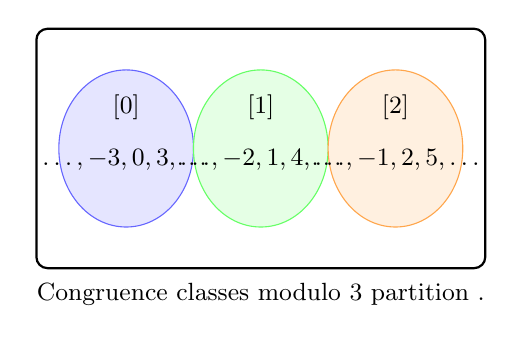
\begin{tikzpicture}[scale=0.95, every node/.style={font=\small}]
\draw[rounded corners, thick] (-3,-1.6) rectangle (3,1.6);
\draw[fill=blue!10, draw=blue!60] (-1.8,0) ellipse (0.9 and 1.05);
\draw[fill=green!10, draw=green!60] (0,0) ellipse (0.9 and 1.05);
\draw[fill=orange!12, draw=orange!70] (1.8,0) ellipse (0.9 and 1.05);
\node at (-1.8,0.55) {$[0]$};
\node at (0,0.55) {$[1]$};
\node at (1.8,0.55) {$[2]$};
\node at (-1.8,-0.15) {$\ldots,-3,0,3,\ldots$};
\node at (0,-0.15) {$\ldots,-2,1,4,\ldots$};
\node at (1.8,-0.15) {$\ldots,-1,2,5,\ldots$};
\node at (0,-1.95) {Congruence classes modulo $3$ partition $\Z$.};
\end{tikzpicture}
\end{center}

The picture suggests two crucial facts:

\begin{itemize}
\item every integer belongs to one of the classes,
\item two classes are either identical or disjoint.
\end{itemize}

Those facts are not special to modulo $3$. They follow from reflexive, symmetric, and transitive. This is one reason equivalence relations are so useful: they turn a relation into a classification system.

\begin{trapbox}
False intuition: equivalence means equality. Better intuition: equivalence means equality after choosing what differences to ignore. Fractions, congruence classes, cosets, projective points, and quotient spaces all use this idea.
\end{trapbox}

\subsection{Common traps with relation properties}

\begin{trapbox}
Symmetric and reflexive are different. Symmetric says relations can be reversed when they occur. It does not say every element is related to itself. A relation may be symmetric but not reflexive.
\end{trapbox}

For example, on $\Z$, define $aRb$ if $a+b=0$. This relation is symmetric: if $a+b=0$, then $b+a=0$. But it is not reflexive, because $a+a=0$ is not true for every integer $a$.

\begin{trapbox}
Transitive does not mean ``eventually connected somehow.'' It means every two-step chain collapses to a one-step relation.
\end{trapbox}

The relation ``is a friend of'' may be symmetric in an idealized social network, but it is not transitive. Your friend's friend need not be your friend.

\subsection{Equivalence relations}

\begin{definition}
A relation $\sim$ on a set $A$ is an \emph{equivalence relation} if it is reflexive, symmetric, and transitive.
\end{definition}

An equivalence relation is a mathematically controlled version of sameness. It does not mean the objects are literally identical. It means they are the same with respect to a chosen feature.

Examples:

\begin{enumerate}
\item On $\Z$, $a\sim b$ if $a-b$ is even. This means $a$ and $b$ have the same parity.
\item On triangles, $T_1\sim T_2$ if $T_1$ is similar to $T_2$. This means they have the same shape, ignoring size.
\item On strings, $s\sim t$ if $s$ and $t$ have the same length.
\item On people, $x\sim y$ if $x$ and $y$ have the same birth year.
\item On ordered pairs of integers with second coordinate nonzero, $(a,b)\sim(c,d)$ if $ad=bc$. This is the relation behind rational numbers.
\end{enumerate}

\begin{intuitionbox}
An equivalence relation says: for the question we are currently asking, these objects count as the same.
\end{intuitionbox}

\subsection{Equivalence classes}

Once we have an equivalence relation, every element has a class around it.

\begin{definition}
Let $\sim$ be an equivalence relation on $A$. The \emph{equivalence class} of $a\in A$ is
\[
[a]=\{x\in A:x\sim a\}.
\]
\end{definition}

For the same-parity relation on $\Z$,
\[
[0]=\{\ldots,-4,-2,0,2,4,\ldots\}
\]
and
\[
[1]=\{\ldots,-3,-1,1,3,5,\ldots\}.
\]
There are only two equivalence classes: the even integers and the odd integers. Notice that $[0]=[2]=[-10]$ and $[1]=[3]=[-7]$.

An equivalence class is not a single object. It is a set of objects. The notation $[a]$ means ``the class represented by $a$.''

\begin{trapbox}
Do not confuse $a$ with $[a]$. The element $a$ belongs to the original set $A$. The class $[a]$ is a subset of $A$.
\end{trapbox}

\subsection{The class theorem}

The key theorem about equivalence classes is that they either match exactly or do not overlap at all.

\begin{theorem}
Let $\sim$ be an equivalence relation on $A$. For any $a,b\in A$, either $[a]=[b]$ or $[a]\cap[b]=\emptyset$.
\end{theorem}

\begin{proof}
Let $a,b\in A$. Suppose $[a]\cap[b]\neq\emptyset$. We will prove $[a]=[b]$.

Since $[a]\cap[b]\neq\emptyset$, choose $x\in[a]\cap[b]$. Then $x\in[a]$ and $x\in[b]$, so $x\sim a$ and $x\sim b$.

Because $x\sim a$, symmetry gives $a\sim x$. Since $a\sim x$ and $x\sim b$, transitivity gives $a\sim b$.

Now we prove the two inclusions.

First, let $y\in[a]$. Then $y\sim a$. Since $a\sim b$, transitivity gives $y\sim b$. Hence $y\in[b]$. Therefore $[a]\subseteq[b]$.

Second, let $y\in[b]$. Then $y\sim b$. From $a\sim b$, symmetry gives $b\sim a$. Since $y\sim b$ and $b\sim a$, transitivity gives $y\sim a$. Hence $y\in[a]$. Therefore $[b]\subseteq[a]$.

Thus $[a]=[b]$. We have shown that if the classes overlap, they are equal. Therefore two equivalence classes are either equal or disjoint.
\end{proof}

This theorem is one of the first examples of a very common mathematical move: instead of trying to understand every element individually, we organize the whole set into blocks.

\subsection{Partitions}

\begin{definition}
A \emph{partition} of a set $A$ is a collection of nonempty subsets of $A$ such that every element of $A$ belongs to exactly one subset in the collection.
\end{definition}

A partition is a clean division of a set into non-overlapping blocks. The months partition the days of a year. The even and odd integers partition $\Z$. Letter grades partition students into groups, at least for one course.

Equivalence relations and partitions are two languages for the same idea.

\begin{theorem}
Every equivalence relation on $A$ determines a partition of $A$ into equivalence classes.
\end{theorem}

\begin{proof}
Let $\sim$ be an equivalence relation on $A$. Consider the collection of all equivalence classes
\[
A/{\sim}=\{[a]:a\in A\}.
\]
Each class is nonempty, because reflexivity gives $a\sim a$, so $a\in[a]$.

Every element of $A$ belongs to some class: if $a\in A$, then $a\in[a]$.

Finally, by the previous theorem, two equivalence classes are either equal or disjoint. Therefore every element belongs to exactly one distinct class. Hence the equivalence classes form a partition of $A$.
\end{proof}

Conversely, every partition defines an equivalence relation: say two elements are related exactly when they belong to the same block.

\begin{labbox}
Let $\mathcal{P}$ be a partition of $A$. Define $a\sim b$ if $a$ and $b$ lie in the same block of $\mathcal{P}$. Prove that $\sim$ is reflexive, symmetric, and transitive. The only subtle part is transitivity: if $a$ and $b$ are in one block and $b$ and $c$ are in one block, why must those two blocks be the same?
\end{labbox}

\subsection{Quotient sets}

The set of equivalence classes is called a quotient set.

\begin{definition}
If $\sim$ is an equivalence relation on $A$, the \emph{quotient set} of $A$ by $\sim$ is
\[
A/{\sim}=\{[a]:a\in A\}.
\]
\end{definition}

The quotient set is the set whose elements are the blocks, not the original objects. This is a conceptual leap. We take a collection of objects and compress each equivalence class into a single new object.

For same parity,
\[
\Z/{\sim}=\{[0],[1]\}.
\]
This quotient has two elements.

For congruence modulo $n$, define
\[
a\equiv b\pmod n\quad\text{if and only if}\quad n\mid(a-b).
\]
Then
\[
\Z/n\Z=\{[0],[1],\ldots,[n-1]\}.
\]
The quotient $\Z/n\Z$ is the mathematical home of clock arithmetic.

\begin{historybox}
Congruence notation was introduced by Carl Friedrich Gauss in \emph{Disquisitiones Arithmeticae} in 1801. Gauss gave number theory a language in which remainders could be treated structurally, not merely as leftovers after division.
\end{historybox}

\subsection{Well-defined operations}

Quotients become powerful when we define operations on classes. For example, in $\Z/n\Z$ we want
\[
[a]+[b]=[a+b].
\]
But this raises a serious question. The class $[a]$ has many representatives. If $a'$ is another representative of $[a]$ and $b'$ is another representative of $[b]$, do we get the same answer?

This is the issue of being well-defined.

\begin{definition}
An operation or function on equivalence classes is \emph{well-defined} if its value does not depend on the choice of representatives.
\end{definition}

\begin{theorem}
Addition modulo $n$ is well-defined: if $a\equiv a'\pmod n$ and $b\equiv b'\pmod n$, then
\[
a+b\equiv a'+b'\pmod n.
\]
\end{theorem}

\begin{proof}
Assume $a\equiv a'\pmod n$ and $b\equiv b'\pmod n$. Then $n\mid(a-a')$ and $n\mid(b-b')$. So there are integers $r,s$ such that
\[
a-a'=nr,\qquad b-b'=ns.
\]
Adding gives
\[
(a+b)-(a'+b')=(a-a')+(b-b')=nr+ns=n(r+s).
\]
Since $r+s\in\Z$, we have $n\mid((a+b)-(a'+b'))$. Hence
\[
a+b\equiv a'+b'\pmod n.
\]
Therefore the rule $[a]+[b]=[a+b]$ is well-defined.
\end{proof}

\begin{trapbox}
When defining something on equivalence classes, never prove only that the formula makes sense for one representative. You must prove that changing representatives does not change the class of the answer.
\end{trapbox}

\subsection{Rational numbers as a quotient}

Fractions hide an equivalence relation. The symbols
\[
\frac12,\quad \frac24,\quad \frac36,\quad \frac{-5}{-10}
\]
are different pairs of integers, but they represent the same rational number.

Let
\[
S=\{(a,b)\in\Z\times\Z:b\neq0\}.
\]
Define a relation on $S$ by
\[
(a,b)\sim(c,d)\quad\text{if and only if}\quad ad=bc.
\]
This relation says that two fractions are equal after cross multiplication.

\begin{theorem}
The relation $\sim$ on $S$ defined by $(a,b)\sim(c,d)$ if $ad=bc$ is an equivalence relation.
\end{theorem}

\begin{proof}
Reflexive: Let $(a,b)\in S$. Then $ab=ba$, so $(a,b)\sim(a,b)$.

Symmetric: Suppose $(a,b)\sim(c,d)$. Then $ad=bc$. Since equality is symmetric, $bc=ad$, which is the same as $cb=da$. Hence $(c,d)\sim(a,b)$.

Transitive: Suppose $(a,b)\sim(c,d)$ and $(c,d)\sim(e,f)$. Then
\[
ad=bc,\qquad cf=de.
\]
We want to prove $af=be$. Since $d\neq0$, multiply the desired comparison through by $d$. From $ad=bc$, multiply by $f$:
\[
adf=bcf.
\]
From $cf=de$, multiply by $b$:
\[
bcf=bde.
\]
Thus $adf=bde$. Since $d\neq0$ and we are working in integers, cancellation gives $af=be$. Hence $(a,b)\sim(e,f)$.

Therefore $\sim$ is an equivalence relation.
\end{proof}

The rational number $\frac{a}{b}$ is really the equivalence class of the pair $(a,b)$. In ordinary arithmetic we usually suppress the class notation because it would be exhausting to write it every time. But the quotient viewpoint explains why $\frac12=\frac24$ without pretending the ordered pairs $(1,2)$ and $(2,4)$ are identical.

\subsection{Relations as data and structure}

In a database, a relation is often represented as a table. In graph theory, a relation is represented by edges. In algebra, a congruence relation allows quotient structures. In topology, identifying points by an equivalence relation creates quotient spaces. In computer science, equivalence relations appear in union-find data structures, compiler optimization, type inference, minimization of automata, and equality saturation.

The same mathematical structure keeps appearing because many problems ask the same question:

\begin{quote}
Which objects should be treated as indistinguishable for this purpose?
\end{quote}

\begin{walkbox}
Think of three situations from daily life where different objects are treated as the same: tickets for the same seat type, files with the same extension, products with the same SKU, people in the same time zone. What is the underlying equivalence relation? What are the equivalence classes?
\end{walkbox}

\subsection{Proof lab: building a quotient}

\begin{labbox}
Let $R$ be the relation on $\R^2$ defined by
\[
(x,y)R(u,v)\quad\text{if and only if}\quad x^2+y^2=u^2+v^2.
\]
\begin{enumerate}
\item Prove that $R$ is an equivalence relation.
\item Describe the equivalence class of $(1,0)$ geometrically.
\item Describe the quotient set $\R^2/R$ in plain language.
\item If you wanted to represent each class by a single number, which number would you choose?
\end{enumerate}
\end{labbox}

\subsection{Exercises}

\begin{enumerate}
\item On $\Z$, define $aRb$ if $a-b$ is divisible by $5$. Prove that $R$ is an equivalence relation and list the five equivalence classes.
\item On $\R$, define $xRy$ if $|x-y|<1$. Which of reflexive, symmetric, and transitive hold?
\item On $\pow(X)$, define $A\,R\,B$ if $A\cap C=B\cap C$ for a fixed subset $C\subseteq X$. Prove that $R$ is an equivalence relation.
\item Let $f:A\to B$ be a function. Define $a\sim a'$ if $f(a)=f(a')$. Prove that $\sim$ is an equivalence relation on $A$.
\item For the relation in the previous exercise, describe the equivalence classes in terms of inverse images.
\item Give an example of a relation that is reflexive and symmetric but not transitive.
\item Give an example of a relation that is symmetric and transitive but not reflexive on its whole set.
\item Explain why the equality relation on any set is an equivalence relation.
\item Explain why the universal relation $A\times A$ is an equivalence relation.
\item Let $A=\{1,2,3,4\}$ and partition it as $\{\{1,4\},\{2\},\{3\}\}$. Write the associated equivalence relation as a set of ordered pairs.
\end{enumerate}

\subsection{Kernel equivalence of a function}

One of the most important sources of equivalence relations is a function. Let
\[
f:A\to B.
\]
Define a relation on $A$ by
\[
a\sim a'\quad\text{if and only if}\quad f(a)=f(a').
\]
This says that two inputs are equivalent when the function cannot tell them apart.

\begin{theorem}
For every function $f:A\to B$, the relation $a\sim a'$ if $f(a)=f(a')$ is an equivalence relation on $A$.
\end{theorem}

\begin{proof}
Reflexive: Let $a\in A$. Since $f(a)=f(a)$, we have $a\sim a$.

Symmetric: Suppose $a\sim a'$. Then $f(a)=f(a')$. By symmetry of equality, $f(a')=f(a)$, so $a'\sim a$.

Transitive: Suppose $a\sim a'$ and $a'\sim a''$. Then
\[
f(a)=f(a')\quad\text{and}\quad f(a')=f(a'').
\]
By transitivity of equality, $f(a)=f(a'')$. Hence $a\sim a''$.

Thus $\sim$ is an equivalence relation.
\end{proof}

The equivalence class of $a$ is
\[
[a]=\{x\in A:f(x)=f(a)\}.
\]
This is exactly the inverse image of the one-point set $\{f(a)\}$:
\[
[a]=f^{-1}(\{f(a)\}).
\]
These classes are sometimes called the fibers of $f$. The quotient $A/{\sim}$ is the set of fibers.

\begin{intuitionbox}
A function partitions its domain according to output. Injective functions have tiny fibers, each with one element. Non-injective functions merge several inputs into the same fiber.
\end{intuitionbox}

Example: Let $f:\R\to\R$ be $f(x)=x^2$. Then
\[
x\sim y\quad\text{if and only if}\quad x^2=y^2.
\]
The class of $3$ is $\{3,-3\}$. The class of $0$ is $\{0\}$. The quotient remembers absolute value rather than sign.

This viewpoint explains one reason equivalence relations matter in algebra. A homomorphism often collapses a structure by identifying elements with the same image. The associated equivalence relation records exactly what was collapsed.

\subsection{Canonical representatives}

After forming a quotient, it is often convenient to choose one representative from each equivalence class. For congruence modulo $n$, the standard representatives are
\[
0,1,\ldots,n-1.
\]
Every integer is congruent to exactly one of these.

But representatives are a convenience, not the quotient itself. In $\Z/5\Z$, the class $[2]$ can be represented by
\[
2,\ 7,\ -3,\ 12,\ -8,\ldots
\]
The object is the whole class. The representative is a name tag.

\begin{trapbox}
When computing in a quotient, reducing to a preferred representative is allowed only after the operation on classes is known to be well-defined.
\end{trapbox}

\begin{labbox}
Let $f:\R\to[0,\infty)$ be $f(x)=|x|$.
\begin{enumerate}
\item Describe the equivalence relation induced by $f$.
\item Describe the equivalence class of $0$.
\item Describe the equivalence class of $5$.
\item Explain why the quotient $\R/{\sim}$ can be represented by $[0,\infty)$.
\item What information is lost when passing from $x$ to $|x|$?
\end{enumerate}
\end{labbox}

\newpage
\section{Orders}

Order relations compare objects by rank, size, inclusion, refinement, information, divisibility, or dependency. The familiar order $\leq$ on numbers is only one example. Once we leave the number line, ordering becomes subtler. Some objects may be comparable, while others may not.

\begin{focusbox}
An order relation is a relation that lets us compare objects without necessarily forcing every pair into a single line.
\end{focusbox}

\subsection{Antisymmetry}

Equivalence relations used reflexive, symmetric, and transitive. Orders usually replace symmetry with antisymmetry.

\begin{definition}
A relation $R$ on a set $A$ is \emph{antisymmetric} if
\[
\forall a,b\in A,\ (aRb\text{ and }bRa)\Rightarrow a=b.
\]
\end{definition}

Antisymmetry does not mean ``not symmetric.'' It means that two different elements cannot be related in both directions.

For $\leq$ on $\R$, if $a\leq b$ and $b\leq a$, then $a=b$. Thus $\leq$ is antisymmetric.

For divisibility on positive integers, if $a\mid b$ and $b\mid a$, then $a=b$. Thus divisibility is antisymmetric on $\N^+=\{1,2,3,\ldots\}$.

For subset inclusion, if $A\subseteq B$ and $B\subseteq A$, then $A=B$. Thus $\subseteq$ is antisymmetric.

\begin{trapbox}
Antisymmetric does not say that $aRb$ prevents $bRa$ in every case. It allows both directions when $a=b$.
\end{trapbox}

\subsection{Partial orders}

\begin{definition}
A relation $\preceq$ on a set $P$ is a \emph{partial order} if it is reflexive, antisymmetric, and transitive. A set equipped with a partial order is called a \emph{partially ordered set}, or \emph{poset}.
\end{definition}

The word ``partial'' means not every pair must be comparable.

Examples:

\begin{enumerate}
\item $(\R,\leq)$ is a poset.
\item $(\pow(X),\subseteq)$ is a poset.
\item Positive integers ordered by divisibility form a poset.
\item Tasks in a project ordered by ``must be completed before'' can form a poset after adding reflexive self-comparison.
\item Subspaces of a vector space ordered by inclusion form a poset.
\end{enumerate}

\subsection{Worked proof: inclusion is a partial order}

\begin{theorem}
For any set $X$, the relation $\subseteq$ is a partial order on $\pow(X)$.
\end{theorem}

\begin{proof}
Reflexive: Let $A\in\pow(X)$. Every element of $A$ is an element of $A$, so $A\subseteq A$.

Antisymmetric: Let $A,B\in\pow(X)$ and suppose $A\subseteq B$ and $B\subseteq A$. To prove $A=B$, use extensionality. If $x\in A$, then $x\in B$ because $A\subseteq B$. If $x\in B$, then $x\in A$ because $B\subseteq A$. Thus $A$ and $B$ have exactly the same elements, so $A=B$.

Transitive: Let $A,B,C\in\pow(X)$ and suppose $A\subseteq B$ and $B\subseteq C$. If $x\in A$, then $x\in B$, and then $x\in C$. Hence $A\subseteq C$.

Therefore $\subseteq$ is reflexive, antisymmetric, and transitive, so it is a partial order.
\end{proof}

\subsection{Comparability}

In a poset $(P,\preceq)$, two elements $a,b\in P$ are \emph{comparable} if
\[
a\preceq b\quad\text{or}\quad b\preceq a.
\]
They are incomparable if neither relation holds.

In $(\pow(\{1,2,3\}),\subseteq)$, the sets $\{1\}$ and $\{1,2\}$ are comparable because $\{1\}\subseteq\{1,2\}$. But $\{1\}$ and $\{2\}$ are incomparable because neither is a subset of the other.

In divisibility, $3$ and $12$ are comparable because $3\mid12$. But $6$ and $10$ are incomparable: neither divides the other.

\begin{intuitionbox}
A partial order is not necessarily a line. It is often a network of constraints. Some elements sit above others, but many pairs may live on separate branches.
\end{intuitionbox}

\subsection{Total orders}

\begin{definition}
A partial order $\preceq$ on $P$ is a \emph{total order} if every pair of elements is comparable:
\[
\forall a,b\in P,\ a\preceq b\text{ or }b\preceq a.
\]
\end{definition}

The usual order $\leq$ on $\R$ is total. For any real numbers $a$ and $b$, either $a\leq b$ or $b\leq a$.

Subset inclusion is usually not total. If $X$ has at least two distinct elements $x$ and $y$, then $\{x\}$ and $\{y\}$ are incomparable.

\begin{trapbox}
Do not assume every order behaves like the number line. Many important orders are partial, not total.
\end{trapbox}

\subsection{Strict orders}

Sometimes we use strict comparison, such as $<$ instead of $\leq$.

\begin{definition}
A relation $\prec$ on $P$ is a \emph{strict partial order} if it is irreflexive and transitive. Irreflexive means
\[
\forall a\in P,\ \neg(a\prec a).
\]
\end{definition}

The relation $<$ on $\R$ is irreflexive and transitive. The relation $\subsetneq$ on $\pow(X)$ is also irreflexive and transitive.

Strict and non-strict orders are closely related. From a partial order $\preceq$, define
\[
a\prec b\quad\text{if and only if}\quad a\preceq b\text{ and }a\neq b.
\]
This gives the associated strict order.

From many strict orders, define
\[
a\preceq b\quad\text{if and only if}\quad a\prec b\text{ or }a=b.
\]
This gives the associated non-strict order.

\subsection{Hasse diagrams}

Finite posets can often be drawn with Hasse diagrams. A Hasse diagram places larger elements higher and draws edges only for immediate cover relations, leaving out reflexive loops and edges implied by transitivity.

For divisibility among $\{1,2,3,6\}$:

\[
\begin{array}{c}
6\\
/ \ \backslash\\
2\quad 3\\
\backslash\ /\\
1
\end{array}
\]

The diagram says $1\mid2$, $1\mid3$, $2\mid6$, and $3\mid6$. It also implies $1\mid6$ by transitivity, so we do not draw a direct edge from $1$ to $6$ in the Hasse diagram.

\subsection{Minimal, maximal, least, and greatest}

Order language becomes precise because there are several kinds of extremal elements.

\begin{definition}
Let $(P,\preceq)$ be a poset and let $S\subseteq P$.
\begin{itemize}
\item An element $m\in S$ is \emph{minimal} in $S$ if there is no $s\in S$ with $s\prec m$.
\item An element $M\in S$ is \emph{maximal} in $S$ if there is no $s\in S$ with $M\prec s$.
\item An element $\ell\in S$ is \emph{least} in $S$ if $\ell\preceq s$ for every $s\in S$.
\item An element $g\in S$ is \emph{greatest} in $S$ if $s\preceq g$ for every $s\in S$.
\end{itemize}
\end{definition}

Least implies minimal. Greatest implies maximal. But minimal does not necessarily imply least, and maximal does not necessarily imply greatest.

Consider $S=\{\{1\},\{2\}\}$ inside $\pow(\{1,2\})$ ordered by $\subseteq$. Both $\{1\}$ and $\{2\}$ are minimal. Neither is least, because neither is a subset of the other.

\begin{trapbox}
``Minimal'' means nothing is strictly below it. ``Least'' means it is below everything. In a partial order these are not the same.
\end{trapbox}

\subsection{Upper bounds and suprema}

\begin{definition}
Let $(P,\preceq)$ be a poset and $S\subseteq P$. An element $u\in P$ is an \emph{upper bound} for $S$ if
\[
\forall s\in S,\ s\preceq u.
\]
A \emph{least upper bound}, or \emph{supremum}, is an upper bound $u$ such that $u\preceq v$ for every upper bound $v$ of $S$.
\end{definition}

Similarly, a lower bound lies below every element of $S$, and a greatest lower bound is called an infimum.

In $\R$ with the usual order, the set $(0,1)$ has many upper bounds: $1$, $2$, $100$. Its least upper bound is $1$, even though $1\notin(0,1)$.

In $\pow(X)$ ordered by $\subseteq$, the supremum of a family of subsets is their union, and the infimum is their intersection.

\begin{theorem}
Let $\mathcal{A}\subseteq\pow(X)$. Under the order $\subseteq$, the least upper bound of $\mathcal{A}$ is $\bigcup_{A\in\mathcal{A}}A$.
\end{theorem}

\begin{proof}
Let
\[
U=\bigcup_{A\in\mathcal{A}}A.
\]
First we show $U$ is an upper bound. If $A\in\mathcal{A}$ and $x\in A$, then by definition of union, $x\in U$. Hence $A\subseteq U$ for every $A\in\mathcal{A}$.

Now let $V$ be any upper bound for $\mathcal{A}$. This means $A\subseteq V$ for every $A\in\mathcal{A}$. We prove $U\subseteq V$. Let $x\in U$. Then $x\in A$ for some $A\in\mathcal{A}$. Since $A\subseteq V$, we get $x\in V$. Therefore $U\subseteq V$.

So $U$ is an upper bound contained in every upper bound. Hence $U$ is the least upper bound.
\end{proof}

\subsection{Divisibility as an order}

Let $\N^+=\{1,2,3,\ldots\}$. Define
\[
a\preceq b\quad\text{if and only if}\quad a\mid b.
\]
This is a partial order.

\begin{proof}
Reflexive: For every $a\in\N^+$, $a\mid a$ because $a=1\cdot a$.

Antisymmetric: Suppose $a\mid b$ and $b\mid a$. Then $b=ak$ and $a=b\ell$ for positive integers $k,\ell$. Substituting gives
\[
a=(ak)\ell=a(k\ell).
\]
Since $a>0$, divide by $a$ to get $1=k\ell$. Since $k,\ell\in\N^+$, we must have $k=\ell=1$. Thus $a=b$.

Transitive: Suppose $a\mid b$ and $b\mid c$. Then $b=ak$ and $c=b\ell$ for positive integers $k,\ell$. Hence $c=(ak)\ell=a(k\ell)$, so $a\mid c$.
\end{proof}

This order is not total. For example, neither $2\mid3$ nor $3\mid2$.

In this order, greatest common divisors and least common multiples can be understood as infima and suprema. The greatest common divisor of $a$ and $b$ is the greatest lower bound of $\{a,b\}$ under divisibility. The least common multiple is the least upper bound.

\begin{historybox}
The Euclidean algorithm is older than modern order theory, but order language reveals what it computes structurally: the greatest element among common divisors. Later algebra generalizes this idea to rings, ideals, lattices, and modules.
\end{historybox}

\subsection{Well-orders}

\begin{definition}
A total order $\leq$ on a set $W$ is a \emph{well-order} if every nonempty subset of $W$ has a least element.
\end{definition}

The natural numbers with their usual order are well-ordered. Every nonempty subset of $\N$ has a least element.

The integers with their usual order are not well-ordered. The subset $\Z$ itself has no least element. The positive real numbers are not well-ordered under the usual order, because $(0,1)$ has no least element.

Well-ordering is the hidden foundation under ordinary induction.

\begin{formalbox}
The well-ordering principle for $\N$ says: every nonempty subset of $\N$ has a least element. It is equivalent, in standard foundations of arithmetic, to mathematical induction.
\end{formalbox}

\subsection{Topological and algebraic echoes}

Orders appear in many later fields.

\begin{itemize}
\item In analysis, the completeness of $\R$ is expressed using least upper bounds.
\item In topology, open sets are ordered by inclusion.
\item In algebra, ideals are ordered by inclusion, and maximal ideals are central.
\item In logic, theories can be ordered by strength.
\item In computer science, program states can be ordered by information content.
\item In category theory, a poset can be viewed as a category with at most one morphism between any two objects.
\end{itemize}

The same theme repeats: structure is not only what objects are, but how they compare.

\subsection{Proof lab: a poset of information}

\begin{labbox}
Let $X$ be a set and let $\mathcal{P}$ be a collection of partitions of $X$. Define $\mathcal{A}\preceq\mathcal{B}$ if every block of $\mathcal{A}$ is contained in some block of $\mathcal{B}$.

This means $\mathcal{A}$ is finer than $\mathcal{B}$: it makes at least as many distinctions.

\begin{enumerate}
\item Prove that $\preceq$ is reflexive.
\item Prove that $\preceq$ is transitive.
\item Think carefully about antisymmetry. If $\mathcal{A}\preceq\mathcal{B}$ and $\mathcal{B}\preceq\mathcal{A}$, why must the partitions be the same?
\item For $X=\{1,2,3\}$, draw the poset of all partitions ordered by refinement.
\end{enumerate}
\end{labbox}

\subsection{Walking prompts}

\begin{walkbox}
Walk through a dependency system you know: course prerequisites, software packages, build steps, recipe steps. Which pairs are comparable? Which are not? What would a least element mean? What would a maximal element mean?
\end{walkbox}

\subsection{Exercises}

\begin{enumerate}
\item Prove that $\leq$ is a total order on $\Z$.
\item Prove that $\subseteq$ is not a total order on $\pow(\{1,2\})$.
\item On $\R$, define $x\preceq y$ if $|x|\leq |y|$. Which partial order properties hold? Which fail?
\item On $\Z$, define $a\preceq b$ if $a\mid b$. Is this antisymmetric on all of $\Z$? Explain.
\item Give a poset with exactly three maximal elements.
\item Give a poset with a unique minimal element that is not least.
\item Find all minimal and maximal elements of $\pow(\{1,2,3\})\setminus\{\emptyset,\{1,2,3\}\}$ under inclusion.
\item Prove that if a least element exists in a poset, it is unique.
\item Prove that if a greatest element exists in a poset, it is unique.
\item Let $S\subseteq\R$ be bounded above. State what it means for $u$ to be $\sup S$ using quantifiers.
\item In $\N^+$ ordered by divisibility, find the infimum and supremum of $\{12,18\}$.
\item Explain why every finite nonempty total order is a well-order.
\end{enumerate}

\subsection{Chains and antichains}

Partial orders become easier to see when we name two opposite patterns.

\begin{definition}
Let $(P,\preceq)$ be a poset. A subset $C\subseteq P$ is a \emph{chain} if every two elements of $C$ are comparable. A subset $A\subseteq P$ is an \emph{antichain} if no two distinct elements of $A$ are comparable.
\end{definition}

In $\pow(\{1,2,3\})$ ordered by inclusion,
\[
\emptyset\subseteq\{1\}\subseteq\{1,2\}\subseteq\{1,2,3\}
\]
is a chain. The set
\[
\{\{1\},\{2\},\{3\}\}
\]
is an antichain.

Chains are the parts of a poset that behave like total orders. Antichains are the parts where comparison fails as much as possible.

\begin{intuitionbox}
A chain is a single line through the poset. An antichain is a horizontal layer of mutually incomparable objects.
\end{intuitionbox}

Chains and antichains matter because they separate two kinds of complexity. A long chain means there are many strict levels of refinement or dependency. A large antichain means there are many independent alternatives that cannot be ranked by the order.

\subsection{Lattices}

Some posets have especially good behavior with respect to pairs.

\begin{definition}
A poset $(L,\preceq)$ is a \emph{lattice} if every pair of elements $a,b\in L$ has a least upper bound and a greatest lower bound.
\end{definition}

The least upper bound of $a$ and $b$ is often called their join and written
\[
a\vee b.
\]
The greatest lower bound is called their meet and written
\[
a\wedge b.
\]

In $\pow(X)$ ordered by inclusion,
\[
A\vee B=A\cup B,\qquad A\wedge B=A\cap B.
\]
Union is the smallest set containing both $A$ and $B$. Intersection is the largest set contained in both.

In positive integers ordered by divisibility,
\[
a\vee b=\operatorname{lcm}(a,b),\qquad a\wedge b=\gcd(a,b).
\]
This is a good example of abstraction paying rent: union/intersection and lcm/gcd are different operations in different settings, but they play the same order-theoretic roles.

\begin{labbox}
Prove that $\pow(X)$ is a lattice under $\subseteq$.
\begin{enumerate}
\item Show $A\cup B$ is an upper bound for $\{A,B\}$.
\item Show every upper bound of $\{A,B\}$ contains $A\cup B$.
\item Show $A\cap B$ is a lower bound for $\{A,B\}$.
\item Show every lower bound of $\{A,B\}$ is contained in $A\cap B$.
\end{enumerate}
\end{labbox}

\subsection{Order-preserving maps}

Functions between ordered sets should sometimes respect order.

\begin{definition}
Let $(P,\preceq_P)$ and $(Q,\preceq_Q)$ be posets. A function $f:P\to Q$ is \emph{order-preserving}, or \emph{monotone}, if
\[
x\preceq_P y\Rightarrow f(x)\preceq_Q f(y).
\]
\end{definition}

Examples:

\begin{enumerate}
\item The function $f:\R\to\R$ given by $f(x)=3x+1$ is order-preserving under the usual order.
\item The function $g:\R\to\R$ given by $g(x)=-x$ is order-reversing, not order-preserving.
\item If $X\subseteq Y$, then the map $\pow(X)\to\pow(Y)$ sending $A$ to $A$ is order-preserving.
\item For positive integers ordered by divisibility, the map $n\mapsto 2n$ is order-preserving.
\end{enumerate}

Order-preserving maps are the structure-respecting maps of order theory. They are to posets what homomorphisms are to algebraic structures and continuous maps are to topological spaces.

\begin{walkbox}
Think of a system where adding information should not reduce what you know: search filters, type constraints, permissions, prerequisites. What is the order? What would an order-preserving function between two such systems mean?
\end{walkbox}

\newpage
\section{Induction}

Mathematical induction is the proof method that turns a local step into an infinite conclusion. It is the formal version of a simple idea: if you can start, and you can always move from one case to the next, then every case is reached.

Beginners often learn induction as a template. The template matters, but induction is more than a template. It is a way of thinking about recursively generated objects, discrete time, algorithms, grammar, trees, sums, divisibility, inequalities, and definitions that refer back to earlier cases.

\begin{focusbox}
Induction proves infinitely many statements by proving two things: the first statement is true, and truth passes from each case to the next.
\end{focusbox}

\subsection{The domino picture}

Imagine infinitely many dominos labeled $0,1,2,3,\ldots$.

To prove all dominos fall, it is enough to prove:

\begin{enumerate}
\item Domino $0$ falls.
\item Whenever domino $n$ falls, domino $n+1$ falls.
\end{enumerate}

The first clause starts the chain. The second clause transmits the chain.

Induction is the same idea for statements. Let $P(n)$ be a statement about $n$. To prove
\[
\forall n\in\N,\ P(n),
\]
we prove:

\begin{enumerate}
\item Base case: $P(0)$ is true.
\item Inductive step: for arbitrary $n\in\N$, if $P(n)$ is true, then $P(n+1)$ is true.
\end{enumerate}

Some books start $\N$ at $1$ instead of $0$. The method is the same. Start at the first value in the claim.

\begin{trapbox}
Always match the base case to the statement. If the theorem says ``for all $n\geq 5$,'' the base case is usually $n=5$, not $n=0$ or $n=1$.
\end{trapbox}

\subsection{The formal principle}

\begin{formalbox}
Principle of mathematical induction: Let $P(n)$ be a predicate on natural numbers. If
\[
P(0)
\]
is true and
\[
\forall n\in\N,\ P(n)\Rightarrow P(n+1)
\]
is true, then
\[
\forall n\in\N,\ P(n)
\]
is true.
\end{formalbox}

The version starting at $1$ says: if $P(1)$ is true and $P(n)\Rightarrow P(n+1)$ for all $n\geq1$, then $P(n)$ is true for all $n\geq1$.

The version starting at $m$ says: if $P(m)$ is true and $P(n)\Rightarrow P(n+1)$ for all $n\geq m$, then $P(n)$ is true for all $n\geq m$.

\subsection{First worked proof: sum of the first $n$ integers}

\begin{theorem}
For every integer $n\geq1$,
\[
1+2+\cdots+n=\frac{n(n+1)}{2}.
\]
\end{theorem}

\begin{proof}
Let $P(n)$ be the statement
\[
1+2+\cdots+n=\frac{n(n+1)}{2}.
\]

Base case: For $n=1$, the left side is $1$, and the right side is
\[
\frac{1(1+1)}{2}=1.
\]
Thus $P(1)$ is true.

Inductive step: Let $n\geq1$ and assume $P(n)$ is true. That is, assume
\[
1+2+\cdots+n=\frac{n(n+1)}{2}.
\]
We must prove $P(n+1)$:
\[
1+2+\cdots+n+(n+1)=\frac{(n+1)(n+2)}{2}.
\]
Starting with the left side,
\[
1+2+\cdots+n+(n+1)
=\frac{n(n+1)}{2}+(n+1)
\]
by the induction hypothesis. Now simplify:
\[
\frac{n(n+1)}{2}+(n+1)
=\frac{n(n+1)+2(n+1)}{2}
=\frac{(n+1)(n+2)}{2}.
\]
So $P(n+1)$ is true.

Therefore, by induction, the formula holds for every integer $n\geq1$.
\end{proof}

The induction hypothesis is not a wish. It is a temporary assumption inside the inductive step. The theorem of induction tells us that if the step works for arbitrary $n$, then the chain is valid.

\subsection{What the induction hypothesis is allowed to do}

In the proof above, we used the induction hypothesis exactly once:
\[
1+2+\cdots+n=\frac{n(n+1)}{2}.
\]
We used it to replace the sum up to $n$ with a formula. Then we added the new term $n+1$.

This is the pattern behind many induction proofs:

\begin{quote}
Use the known case to handle most of the new case, then deal with the new piece.
\end{quote}

\begin{trapbox}
Do not assume $P(n+1)$ in the inductive step. You assume $P(n)$ and prove $P(n+1)$.
\end{trapbox}

\subsection{Induction and recursion}

Induction is proof. Recursion is definition or computation. They are paired because recursive objects are built by base rules and step rules.

For example, define factorial recursively:
\[
0!=1,\qquad (n+1)!=(n+1)n!.
\]
This definition tells us how to build factorial values. Induction tells us how to prove facts about all of them.

\begin{theorem}
For every $n\geq1$, $n!\geq 2^{n-1}$.
\end{theorem}

\begin{proof}
Let $P(n)$ be the statement $n!\geq2^{n-1}$.

Base case: For $n=1$, we have $1!=1$ and $2^{0}=1$, so $1!\geq2^0$.

Inductive step: Let $n\geq1$ and assume $n!\geq2^{n-1}$. We need to prove
\[
(n+1)!\geq2^n.
\]
Since $n+1\geq2$, we have
\[
(n+1)!=(n+1)n!\geq2n!.
\]
By the induction hypothesis, $n!\geq2^{n-1}$, so
\[
2n!\geq2\cdot2^{n-1}=2^n.
\]
Thus $(n+1)!\geq2^n$.

Therefore $n!\geq2^{n-1}$ for every $n\geq1$.
\end{proof}

\subsection{Proving divisibility}

Induction is especially useful when a statement changes predictably as $n$ increases.

\begin{theorem}
For every $n\geq1$, the number $n^3-n$ is divisible by $3$.
\end{theorem}

\begin{proof}
Let $P(n)$ be the statement $3\mid(n^3-n)$.

Base case: For $n=1$,
\[
1^3-1=0,
\]
and $3\mid0$. So $P(1)$ is true.

Inductive step: Let $n\geq1$ and assume $3\mid(n^3-n)$. We must prove
\[
3\mid((n+1)^3-(n+1)).
\]
Compute:
\[
(n+1)^3-(n+1)
=n^3+3n^2+3n+1-n-1
=n^3-n+3n^2+3n.
\]
So
\[
(n+1)^3-(n+1)=(n^3-n)+3(n^2+n).
\]
The first term is divisible by $3$ by the induction hypothesis, and the second term is visibly divisible by $3$. Therefore their sum is divisible by $3$.

Thus $P(n+1)$ is true, and induction proves the claim.
\end{proof}

This theorem can also be proved without induction by factoring:
\[
n^3-n=n(n-1)(n+1),
\]
the product of three consecutive integers. Among three consecutive integers, one is divisible by $3$. The two proofs reveal different things. The induction proof reveals stability from $n$ to $n+1$. The factoring proof reveals a structural divisibility reason.

\begin{intuitionbox}
When you find a non-inductive proof of a theorem first proved by induction, do not treat one proof as wasted. Different proofs often expose different mechanisms.
\end{intuitionbox}

\subsection{Induction with inequalities}

Inequality proofs by induction require care because algebraic transformations may need side conditions such as positivity.

\begin{theorem}
For every integer $n\geq4$,
\[
2^n\geq n^2.
\]
\end{theorem}

\begin{proof}
Let $P(n)$ be the statement $2^n\geq n^2$.

Base case: For $n=4$, $2^4=16$ and $4^2=16$, so $P(4)$ is true.

Inductive step: Let $n\geq4$ and assume $2^n\geq n^2$. We must show
\[
2^{n+1}\geq(n+1)^2.
\]
Starting from the induction hypothesis,
\[
2^{n+1}=2\cdot2^n\geq2n^2.
\]
It remains to show
\[
2n^2\geq(n+1)^2.
\]
This inequality is equivalent to
\[
2n^2-(n+1)^2=n^2-2n-1\geq0.
\]
For $n\geq4$,
\[
n^2-2n-1=n(n-2)-1\geq4\cdot2-1=7>0.
\]
Therefore $2n^2\geq(n+1)^2$, and hence
\[
2^{n+1}\geq(n+1)^2.
\]
By induction, $2^n\geq n^2$ for all $n\geq4$.
\end{proof}

\begin{trapbox}
In inequality induction, do not replace a difficult target by a stronger inequality unless you actually prove the stronger inequality. Keep track of the direction of every inequality.
\end{trapbox}

\subsection{Induction with sets}

Induction is not only about formulas. It can prove statements about finite sets.

\begin{theorem}
If $A$ is a finite set with $n$ elements, then $\pow(A)$ has $2^n$ elements.
\end{theorem}

\begin{proof}
We prove by induction on $n$.

Base case: If $n=0$, then $A=\emptyset$. The only subset of $\emptyset$ is $\emptyset$ itself, so $\pow(A)$ has $1=2^0$ element.

Inductive step: Assume every set with $n$ elements has $2^n$ subsets. Let $A$ be a set with $n+1$ elements. Choose an element $a\in A$, and let $B=A\setminus\{a\}$. Then $B$ has $n$ elements.

Every subset of $A$ falls into exactly one of two types:

\begin{itemize}
\item subsets that do not contain $a$,
\item subsets that do contain $a$.
\end{itemize}

The subsets that do not contain $a$ are exactly the subsets of $B$, so there are $2^n$ of them by the induction hypothesis.

The subsets that do contain $a$ are obtained by taking a subset $C\subseteq B$ and forming $C\cup\{a\}$. This gives one subset of $A$ containing $a$ for each subset of $B$, so there are also $2^n$ of them.

Therefore
\[
|\pow(A)|=2^n+2^n=2^{n+1}.
\]
By induction, every finite set with $n$ elements has $2^n$ subsets.
\end{proof}

This proof is recursive thinking: to understand subsets of a set with $n+1$ elements, remove one element and use the subsets of the smaller set.

\subsection{Induction and algorithms}

Algorithm correctness proofs often use induction. A loop invariant is an induction statement in disguise. It says: after $n$ iterations, some property holds.

Suppose an algorithm computes the sum of a list $a_1,\ldots,a_m$:

\[
\begin{array}{l}
s:=0\\
\text{for }i=1\text{ to }m:\\
\qquad s:=s+a_i
\end{array}
\]

The loop invariant is:
\[
\text{After }k\text{ iterations, }s=a_1+\cdots+a_k.
\]

Base case: before the loop, $k=0$ and $s=0$, the empty sum.

Step: if after $k$ iterations $s=a_1+\cdots+a_k$, then after the next iteration,
\[
s=(a_1+\cdots+a_k)+a_{k+1}.
\]
So the invariant holds for $k+1$.

At the end, $k=m$, so $s=a_1+\cdots+a_m$.

\begin{intuitionbox}
Induction is the proof version of a loop invariant: establish the initial state, prove preservation, then conclude the final property.
\end{intuitionbox}

\subsection{False induction proofs}

Here is a famous false proof:

\begin{quote}
Claim: All horses are the same color.
\end{quote}

The proposed induction is on the number $n$ of horses in a group. For $n=1$, all horses in a one-horse group have the same color. Assume every group of $n$ horses has the same color. Given $n+1$ horses, remove the last horse. The first $n$ have the same color. Then remove the first horse. The last $n$ have the same color. Since these two groups overlap, all $n+1$ horses have the same color.

The flaw occurs when moving from $n=1$ to $n=2$. The two one-horse groups do not overlap. Without overlap, there is no bridge carrying color information from one horse to the other.

\begin{trapbox}
In an induction proof, the inductive step must work for every allowed $n$. A step that works only after some later value does not connect the base case to the chain.
\end{trapbox}

\subsection{Proof lab: diagnose an induction}

\begin{labbox}
A student tries to prove that $n^2+n+1$ is even for all $n\geq1$.

They write: ``Base case: for $n=1$, $1^2+1+1=3$, which is odd. Inductive step: assume $n^2+n+1$ is even. Then
\[
(n+1)^2+(n+1)+1=n^2+3n+3.
\]
This is close to $n^2+n+1$, so it is also even.''

\begin{enumerate}
\item What is wrong with the claim?
\item What is wrong with the base case?
\item What is wrong with the phrase ``close to''?
\item Find a true statement similar to this one and prove it.
\end{enumerate}
\end{labbox}

\subsection{Historical connections}

\begin{historybox}
Inductive reasoning appears implicitly in ancient mathematics, but explicit formulations developed over time. Pascal used an argument recognizable as induction in work related to the arithmetic triangle. Modern axiomatizations of arithmetic, such as the Peano axioms, place induction at the foundation of the natural numbers.
\end{historybox}

Induction also connects to the philosophical question: what are the natural numbers? One answer is operational. The natural numbers are generated from a starting point by repeatedly applying a successor operation. Induction says that any property containing the start and closed under successor contains all natural numbers.

\subsection{Writing induction clearly}

A clean induction proof usually includes:

\begin{enumerate}
\item The predicate $P(n)$.
\item The base case.
\item The induction hypothesis.
\item The target $P(n+1)$.
\item The argument proving the target.
\item The final sentence invoking induction.
\end{enumerate}

The target matters. Many confused proofs never state what must be proved in the step. Before doing algebra, write the desired statement for $n+1$.

\begin{walkbox}
While walking, practice saying the skeleton aloud: ``I prove $P(n)$ by induction. First $P(m)$. Now assume $P(n)$ for arbitrary $n\geq m$. I must prove $P(n+1)$.'' The rhythm is part of the discipline.
\end{walkbox}

\subsection{Exercises}

\begin{enumerate}
\item Prove that for all $n\geq1$,
\[
1+3+5+\cdots+(2n-1)=n^2.
\]
\item Prove that for all $n\geq1$,
\[
2+4+6+\cdots+2n=n(n+1).
\]
\item Prove that for all $n\geq1$,
\[
1^2+2^2+\cdots+n^2=\frac{n(n+1)(2n+1)}{6}.
\]
\item Prove that $5\mid(6^n-1)$ for every $n\geq1$.
\item Prove that $3\mid(4^n-1)$ for every $n\geq1$.
\item Prove that $n<2^n$ for every $n\geq1$.
\item Prove that $3^n\geq2n+1$ for every $n\geq0$.
\item Prove that a set with $n$ elements has $n(n-1)/2$ two-element subsets.
\item Let $a_1=1$ and $a_{n+1}=2a_n+1$. Prove that $a_n=2^n-1$ for all $n\geq1$.
\item Let $F_0=0$, $F_1=1$, and $F_{n+2}=F_{n+1}+F_n$. Compute the first eight values and guess a parity pattern. Prove your pattern.
\end{enumerate}

\subsection{Induction as an invariant machine}

A useful way to think about induction is to look for an invariant: something that remains true after each step. The base case establishes the invariant, and the inductive step proves it is preserved.

For example, suppose a process starts with one region in the plane. Each move draws a line segment that starts and ends on existing boundary and splits one existing region into two. After $n$ moves, how many regions are there?

The answer is $n+1$.

\begin{proof}
Let $P(n)$ be the statement: after $n$ valid splitting moves, there are $n+1$ regions.

Base case: Before any moves, there is $1=0+1$ region.

Inductive step: Assume after $n$ moves there are $n+1$ regions. The next valid move splits one existing region into two. All other regions remain unchanged. Therefore the number of regions increases by exactly $1$, giving
\[
(n+1)+1=n+2
\]
regions after $n+1$ moves. This is $P(n+1)$.

By induction, after $n$ moves there are $n+1$ regions.
\end{proof}

This proof is short because the invariant is well chosen. We did not need to know the geometry of every region. We needed only the effect of one move.

\begin{intuitionbox}
Good induction proofs often identify the part of the situation that changes predictably and ignore irrelevant detail.
\end{intuitionbox}

\subsection{Induction and definitions by stages}

Many mathematical sets are defined in stages. For example, define a set $S$ of strings over the alphabet $\{a,b\}$ as follows:

\begin{enumerate}
\item The empty string $\epsilon$ belongs to $S$.
\item If $w\in S$, then $awb\in S$.
\end{enumerate}

The strings in $S$ are
\[
\epsilon,\ ab,\ aabb,\ aaabbb,\ldots
\]
Every string in $S$ has the same number of $a$'s and $b$'s, with all the $a$'s first.

To prove this, induction follows the construction stages. The base object $\epsilon$ has zero $a$'s and zero $b$'s. If $w$ has equal numbers of $a$'s and $b$'s, then $awb$ has one more of each.

This is the beginning of structural induction. Instead of inducting on a visible number $n$, we induct on how an object is built.

\begin{labbox}
Let $S$ be the smallest set of strings such that $\epsilon\in S$ and whenever $w\in S$, the string $awb$ belongs to $S$.
\begin{enumerate}
\item Prove every string in $S$ has equal numbers of $a$'s and $b$'s.
\item Prove every nonempty string in $S$ starts with $a$ and ends with $b$.
\item Is every string with equal numbers of $a$'s and $b$'s in $S$? Give a counterexample if not.
\end{enumerate}
\end{labbox}

\subsection{When induction is the wrong first tool}

Induction is powerful, but not every statement about natural numbers needs it. Sometimes factoring, parity, modular arithmetic, or a direct combinatorial argument is clearer.

For example, the statement
\[
n^2+n\text{ is even}
\]
can be proved by induction, but the direct proof
\[
n^2+n=n(n+1)
\]
is better: one of two consecutive integers is even.

Choosing proof methods is part of mathematical taste. Induction is best when the statement has a natural ``next case'' structure. If the expression already factors into a known pattern, use the pattern.

\begin{walkbox}
For a theorem about $n$, ask two questions before choosing induction: What changes from $n$ to $n+1$? Is there a direct structural reason that avoids stepping through the natural numbers?
\end{walkbox}

\newpage
\section{Strong Induction}

Ordinary induction lets you use the immediately previous case. Strong induction lets you use all previous cases. Despite the name, it is not logically stronger in standard arithmetic. It is a different packaging of the same principle, and it is often the natural way to prove statements where the current object breaks into smaller pieces of many possible sizes.

\begin{focusbox}
Use strong induction when the proof of $P(n)$ may need $P(k)$ for several earlier values $k<n$, not only $P(n-1)$.
\end{focusbox}

\subsection{The principle}

\begin{formalbox}
Principle of strong induction: Let $P(n)$ be a predicate on integers $n\geq m$. If for every $n\geq m$,
\[
\bigl(P(m)\text{ and }P(m+1)\text{ and }\cdots\text{ and }P(n-1)\bigr)\Rightarrow P(n),
\]
then $P(n)$ holds for every $n\geq m$.
\end{formalbox}

Many presentations separate a base case from the step. A common version says:

\begin{enumerate}
\item Prove $P(m)$.
\item For arbitrary $n>m$, assume $P(k)$ for every $m\leq k<n$, and prove $P(n)$.
\end{enumerate}

Then $P(n)$ holds for all $n\geq m$.

\subsection{Why this is not magic}

Strong induction may feel suspicious because, in the step, we assume many cases. But for a fixed $n$, those are all earlier cases. The proof does not assume the conclusion $P(n)$ itself.

Think of climbing a staircase where each step can be reached from any earlier step, not only the immediately previous one. If you can prove that every step is reachable provided all lower steps are reachable, the staircase is still climbed from the bottom.

\subsection{Equivalence with ordinary induction}

Strong induction and ordinary induction are equivalent over the natural numbers. One way to see this is to define a new predicate
\[
Q(n): P(m),P(m+1),\ldots,P(n)\text{ are all true}.
\]
If ordinary induction proves $Q(n)$ for all $n$, then $P(n)$ is true for all $n$.

Thus strong induction is not a new axiom. It is a convenient proof form.

\subsection{Prime factorization existence}

The classic first use of strong induction is proving that every integer greater than $1$ has a prime factorization.

\begin{definition}
An integer $p>1$ is \emph{prime} if its only positive divisors are $1$ and $p$. An integer $n>1$ is \emph{composite} if $n=ab$ for integers $a,b$ with $1<a<n$ and $1<b<n$.
\end{definition}

\begin{theorem}
Every integer $n>1$ is either prime or can be written as a product of primes.
\end{theorem}

\begin{proof}
We use strong induction on $n$.

Let $P(n)$ be the statement: $n$ is prime or $n$ can be written as a product of primes.

Base case: $n=2$. The number $2$ is prime, so $P(2)$ is true.

Strong inductive step: Let $n>2$ and assume $P(k)$ is true for every integer $k$ with $2\leq k<n$. We prove $P(n)$.

If $n$ is prime, then $P(n)$ is true.

If $n$ is not prime, then since $n>1$, it is composite. So
\[
n=ab
\]
for integers $a,b$ with $1<a<n$ and $1<b<n$.

By the strong induction hypothesis, $P(a)$ and $P(b)$ are true. Therefore each of $a$ and $b$ is either prime or a product of primes. Multiplying those prime factorizations gives a product of primes equal to $n$.

Thus $P(n)$ is true in all cases.

By strong induction, every integer $n>1$ is prime or a product of primes.
\end{proof}

Ordinary induction is awkward here because if $n=ab$, the factors $a$ and $b$ are smaller than $n$, but they are not necessarily $n-1$.

\subsection{The role of smaller subproblems}

Strong induction fits recursive decomposition:

\begin{itemize}
\item A number factors into smaller numbers.
\item A polygon can be cut into a triangle plus a smaller polygon.
\item A full binary tree can be split into smaller left and right subtrees.
\item A string generated by a grammar may contain smaller generated strings.
\item An algorithm on input size $n$ may call itself on inputs of size $\lfloor n/2\rfloor$.
\end{itemize}

When the proof needs smaller pieces whose sizes vary, strong induction is often the clean form.

\subsection{Postage theorem}

\begin{theorem}
Every integer amount of postage $n\geq12$ cents can be formed using only $4$-cent and $5$-cent stamps.
\end{theorem}

\begin{proof}
Let $P(n)$ be the statement that $n$ cents can be formed using $4$-cent and $5$-cent stamps.

We prove four base cases:
\[
12=4+4+4,
\]
\[
13=4+4+5,
\]
\[
14=4+5+5,
\]
\[
15=5+5+5.
\]
So $P(12),P(13),P(14),P(15)$ are true.

Inductive step: Let $n\geq16$ and assume $P(k)$ is true for every $12\leq k<n$. We prove $P(n)$.

Since $n\geq16$, we have $n-4\geq12$. Also $n-4<n$. By the strong induction hypothesis, $n-4$ cents can be formed using $4$-cent and $5$-cent stamps. Add one more $4$-cent stamp to get $n$ cents.

Therefore $P(n)$ is true.

By strong induction, every $n\geq12$ can be formed using $4$-cent and $5$-cent stamps.
\end{proof}

This proof shows why multiple base cases are sometimes necessary. The step moves forward by $4$, so the base cases must cover all residue classes modulo $4$ starting at the threshold.

\begin{trapbox}
If your inductive step proves $P(n)$ from $P(n-d)$, you usually need enough base cases to bridge the gap. One base case may not start every chain.
\end{trapbox}

\subsection{Tiling and recursive structure}

\begin{theorem}
For every $n\geq1$, a $2\times n$ board can be tiled by dominoes in $F_{n+1}$ ways, where $F_1=1$, $F_2=1$, and $F_{k+2}=F_{k+1}+F_k$.
\end{theorem}

\begin{proof}
Let $T(n)$ be the number of domino tilings of a $2\times n$ board. We prove $T(n)=F_{n+1}$.

Base cases: For $n=1$, there is exactly one tiling, using one vertical domino. Thus $T(1)=1=F_2$.

For $n=2$, there are two tilings: two vertical dominoes, or two horizontal dominoes stacked. Thus $T(2)=2=F_3$.

Inductive step: Let $n\geq3$ and assume $T(k)=F_{k+1}$ for all $1\leq k<n$. Consider a tiling of a $2\times n$ board.

Look at the leftmost column. Either it is covered by one vertical domino, leaving a $2\times(n-1)$ board, or it is covered by two horizontal dominoes extending into the second column, leaving a $2\times(n-2)$ board.

These two cases are disjoint and exhaustive. Hence
\[
T(n)=T(n-1)+T(n-2).
\]
By the induction hypothesis,
\[
T(n-1)=F_n,\qquad T(n-2)=F_{n-1}.
\]
Therefore
\[
T(n)=F_n+F_{n-1}=F_{n+1}.
\]
By strong induction, the formula holds for every $n\geq1$.
\end{proof}

The proof is not about algebra first. It is about classifying the first local choice and reducing the rest of the board to smaller boards.

\subsection{Complete induction from well-ordering}

Strong induction can be justified using the well-ordering principle.

\begin{theorem}
Assume every nonempty subset of $\N$ has a least element. Then strong induction holds.
\end{theorem}

\begin{proof}
Let $P(n)$ be a predicate for $n\geq m$. Suppose that for every $n\geq m$, if $P(k)$ holds for all $m\leq k<n$, then $P(n)$ holds.

Assume, for contradiction, that $P(n)$ fails for at least one $n\geq m$. Let
\[
S=\{n\in\N:n\geq m\text{ and }P(n)\text{ is false}\}.
\]
By assumption, $S$ is nonempty. By well-ordering, $S$ has a least element; call it $s$.

Since $s$ is the least counterexample, every integer $k$ with $m\leq k<s$ satisfies $P(k)$. By the induction step hypothesis, $P(s)$ must hold. This contradicts $s\in S$.

Therefore there is no counterexample, and $P(n)$ holds for all $n\geq m$.
\end{proof}

This proof is a model of a common strategy: assume there is a counterexample, choose the least one, and use minimality to make all smaller cases available.

\subsection{Minimal counterexample method}

The minimal counterexample method is strong induction in contradiction clothing.

To prove $P(n)$ for all $n\geq m$:

\begin{enumerate}
\item Suppose the claim is false.
\item Let $s$ be the least counterexample.
\item Use the fact that all smaller cases are true.
\item Derive a contradiction.
\end{enumerate}

This method often feels more natural in number theory.

\begin{theorem}
Every integer $n\geq2$ has a prime divisor.
\end{theorem}

\begin{proof}
Suppose not. Then there is at least one integer $n\geq2$ with no prime divisor. Let $s$ be the least such integer.

If $s$ is prime, then $s$ is a prime divisor of itself, contradiction.

If $s$ is composite, then $s=ab$ with $1<a<s$ and $1<b<s$. Since $a\geq2$ and $a<s$, the minimality of $s$ implies that $a$ has a prime divisor $p$. Since $p\mid a$ and $a\mid s$, we have $p\mid s$. This contradicts the choice of $s$.

Therefore every integer $n\geq2$ has a prime divisor.
\end{proof}

\subsection{Recursive definitions and strong induction}

Some definitions call on earlier values in more than one way. The Fibonacci sequence is the standard example:
\[
F_0=0,\qquad F_1=1,\qquad F_{n+2}=F_{n+1}+F_n.
\]
To prove a property of $F_{n+2}$, one may need both earlier cases $F_{n+1}$ and $F_n$.

\begin{theorem}
For every $n\geq0$, $F_n\leq2^n$.
\end{theorem}

\begin{proof}
We use strong induction.

Base cases: $F_0=0\leq1=2^0$, and $F_1=1\leq2=2^1$.

Inductive step: Let $n\geq2$ and assume $F_k\leq2^k$ for all $0\leq k<n$. Then
\[
F_n=F_{n-1}+F_{n-2}\leq2^{n-1}+2^{n-2}.
\]
Since
\[
2^{n-1}+2^{n-2}=3\cdot2^{n-2}\leq4\cdot2^{n-2}=2^n,
\]
we get $F_n\leq2^n$.

By strong induction, $F_n\leq2^n$ for all $n\geq0$.
\end{proof}

\subsection{Common traps in strong induction}

\begin{trapbox}
Do not say ``assume true for all $n$'' in a strong induction step. Say ``assume true for all $k$ with $m\leq k<n$.'' The bound matters.
\end{trapbox}

\begin{trapbox}
Do not use the case $P(n)$ while proving $P(n)$. Strong induction gives previous cases only, not the current case.
\end{trapbox}

\begin{trapbox}
Check that every smaller value you use lies inside the range where the induction hypothesis applies. If the theorem starts at $n=12$, you cannot invoke the hypothesis at $8$.
\end{trapbox}

\subsection{Proof lab: choose induction type}

\begin{labbox}
For each problem, decide whether ordinary induction or strong induction is more natural. Then write the induction hypothesis and the target statement.

\begin{enumerate}
\item Prove $1+2+\cdots+n=n(n+1)/2$.
\item Prove every integer $n\geq2$ is prime or a product of primes.
\item Prove every $2\times n$ board has a number of domino tilings satisfying $T(n)=T(n-1)+T(n-2)$.
\item Prove $7\mid(8^n-1)$ for every $n\geq1$.
\item Prove every integer $n\geq18$ can be written as $4a+7b$ for some nonnegative integers $a,b$.
\end{enumerate}
\end{labbox}

\subsection{Historical connections}

\begin{historybox}
The natural numbers are not merely a list; they are an inductive structure. Peano's axioms isolate this structure using zero, successor, and induction. Strong induction, recursion, and well-ordering are different faces of the same basic architecture.
\end{historybox}

Modern mathematics extends induction far beyond $\N$. Structural induction proves statements about recursively defined syntax trees. Transfinite induction proves statements over well-ordered sets larger than $\N$. Noetherian induction proves statements in settings where infinite descending chains are impossible.

\subsection{Walking prompts}

\begin{walkbox}
Find something built recursively: a folder tree, a family tree, a parsed expression, a proof, a build dependency graph. What are the base objects? What are the construction rules? What would an induction proof about all such objects look like?
\end{walkbox}

\subsection{Exercises}

\begin{enumerate}
\item Prove that every integer $n\geq2$ is divisible by some prime.
\item Prove that every integer $n\geq2$ can be written as a product of primes.
\item Prove that every integer $n\geq8$ can be written as $3a+5b$ for nonnegative integers $a,b$.
\item Prove that every integer $n\geq18$ can be written as $4a+7b$ for nonnegative integers $a,b$.
\item Let $a_0=1$, $a_1=2$, and $a_n=3a_{n-1}+2a_{n-2}$ for $n\geq2$. Prove $a_n\leq5^n$ for all $n\geq0$.
\item Prove that a convex polygon with $n\geq3$ sides can be triangulated into $n-2$ triangles.
\item Prove that every full binary tree has an odd number of vertices.
\item Use the minimal counterexample method to prove that there is no smallest positive rational number.
\item Explain why the postage theorem with $4$-cent and $5$-cent stamps needs four base cases in the proof given above.
\item Give an example of a theorem where ordinary induction is possible but strong induction is cleaner.
\end{enumerate}

\subsection{Structural induction preview}

Strong induction still uses natural numbers as the measuring device. Structural induction goes one step further: it proves statements about all objects generated by rules.

Consider fully parenthesized expressions built from variables using a binary operation symbol $*$:

\begin{enumerate}
\item Every variable is an expression.
\item If $E$ and $F$ are expressions, then $(E*F)$ is an expression.
\end{enumerate}

Examples:
\[
x,\qquad (x*y),\qquad ((x*y)*z),\qquad (x*(y*z)).
\]

Suppose we want to prove that every expression has one more variable occurrence than operation symbols. Let $v(E)$ be the number of variable occurrences in $E$, and let $o(E)$ be the number of operation symbols in $E$. The claim is
\[
v(E)=o(E)+1.
\]

\begin{proof}
We prove the claim by structural induction on expressions.

Base case: If $E$ is a variable, then $v(E)=1$ and $o(E)=0$, so $v(E)=o(E)+1$.

Recursive step: Suppose $E=(F*G)$, where $F$ and $G$ are expressions satisfying the claim. Thus
\[
v(F)=o(F)+1,\qquad v(G)=o(G)+1.
\]
For $E=(F*G)$, we have
\[
v(E)=v(F)+v(G)
\]
and
\[
o(E)=o(F)+o(G)+1.
\]
Therefore
\[
v(E)=v(F)+v(G)=(o(F)+1)+(o(G)+1)=o(F)+o(G)+2.
\]
But
\[
o(E)+1=(o(F)+o(G)+1)+1=o(F)+o(G)+2.
\]
Hence $v(E)=o(E)+1$.

By structural induction, the claim holds for every expression.
\end{proof}

This proof has the same spirit as strong induction: assume the result for smaller pieces and prove it for the object built from those pieces. The difference is that the construction rules, not just the integer order, guide the proof.

\subsection{Noetherian induction}

A deeper generalization appears when a structure has no infinite descending chains. Suppose a relation $\prec$ means ``is simpler than.'' If there is no endless sequence
\[
x_0\succ x_1\succ x_2\succ\cdots,
\]
then one can often prove a statement for every object by assuming it for all simpler objects.

This is called Noetherian induction. It appears in algebra, rewriting systems, termination proofs, and algebraic geometry.

\begin{historybox}
Emmy Noether's work transformed abstract algebra by emphasizing structural conditions such as chain conditions on ideals. Noetherian arguments often say: a process cannot descend forever, so a minimal counterexample would have to exist, and then it can be contradicted.
\end{historybox}

You do not need Noetherian induction yet, but it is useful to know the direction of travel. Ordinary induction, strong induction, structural induction, and minimal counterexample arguments are part of one family: prove everything by showing that failure cannot first appear.

\begin{labbox}
Let $E$ be the set of expressions built from variables and a binary operation $*$ as above.
\begin{enumerate}
\item Prove that every expression has balanced parentheses.
\item Prove that every expression with at least one operation symbol starts with $($ and ends with $)$.
\item Define the depth of an expression recursively and prove that every expression has finite depth.
\end{enumerate}
\end{labbox}

\newpage
\section{Countability}

Countability is where infinity becomes a precise subject. The central surprise is that infinite sets can have different sizes. Some infinities can be listed, at least in principle. Others cannot.

This chapter begins with a simple question:

\begin{quote}
What does it mean for two sets to have the same number of elements?
\end{quote}

For finite sets, we count. For infinite sets, counting one by one may never end, so we compare sets by functions.

\begin{focusbox}
Two sets have the same size when their elements can be paired perfectly: every element on each side is used exactly once.
\end{focusbox}

\subsection{Same size means bijection}

\begin{definition}
Sets $A$ and $B$ are \emph{equinumerous}, or have the same cardinality, if there exists a bijection $f:A\to B$.
\end{definition}

A bijection is a perfect pairing:

\begin{itemize}
\item injective means no two elements of $A$ are paired with the same element of $B$,
\item surjective means every element of $B$ is paired with something from $A$.
\end{itemize}

For finite sets, this agrees with ordinary counting. For infinite sets, it becomes surprising.

\subsection{The even natural numbers}

Let
\[
E=\{0,2,4,6,\ldots\}.
\]
The function $f:\N\to E$ defined by
\[
f(n)=2n
\]
is a bijection. Therefore $\N$ and the even natural numbers have the same cardinality.

This does not mean $E=\N$. It means the elements can be paired:
\[
0\leftrightarrow0,\quad 1\leftrightarrow2,\quad 2\leftrightarrow4,\quad 3\leftrightarrow6,\ldots
\]

\begin{intuitionbox}
Infinite sets can be the same size as proper subsets of themselves. This is one reason infinity cannot be treated like a very large finite number.
\end{intuitionbox}

\subsection{Countably infinite}

\begin{definition}
A set $A$ is \emph{countably infinite} if there exists a bijection $\N\to A$.
\end{definition}

Equivalently, $A$ is countably infinite if its elements can be listed as
\[
a_0,a_1,a_2,a_3,\ldots
\]
with every element of $A$ appearing exactly once.

A set is \emph{countable} if it is finite or countably infinite.

\begin{trapbox}
``Countable'' does not mean ``small'' in an everyday sense. A countably infinite set is infinite. It means listable by natural numbers.
\end{trapbox}

\subsection{The integers are countable}

The integers extend in both directions:
\[
\ldots,-3,-2,-1,0,1,2,3,\ldots
\]
At first they look bigger than $\N$. But they can be listed:
\[
0,1,-1,2,-2,3,-3,\ldots
\]

One bijection $f:\N\to\Z$ is
\[
f(n)=
\begin{cases}
n/2,&\text{if }n\text{ is even},\\
-(n+1)/2,&\text{if }n\text{ is odd}.
\end{cases}
\]
Then
\[
f(0)=0,\quad f(1)=-1,\quad f(2)=1,\quad f(3)=-2,\quad f(4)=2.
\]
This lists every integer exactly once.

\begin{theorem}
The set $\Z$ is countably infinite.
\end{theorem}

\begin{proof}
Define $f:\N\to\Z$ by
\[
f(n)=
\begin{cases}
n/2,&\text{if }n\text{ is even},\\
-(n+1)/2,&\text{if }n\text{ is odd}.
\end{cases}
\]
We show $f$ is bijective.

Surjective: Let $z\in\Z$. If $z\geq0$, then $z=f(2z)$. If $z<0$, then $z=f(-2z-1)$, since $-2z-1$ is a nonnegative odd integer and
\[
f(-2z-1)=-\frac{(-2z-1)+1}{2}=z.
\]
Thus every integer is hit.

Injective: The even inputs map to nonnegative integers and the odd inputs map to negative integers, so an even input and an odd input cannot have the same output. Among even inputs, $f(2a)=a$, so equality of outputs gives equality of inputs. Among odd inputs, $f(2a+1)=-(a+1)$, so equality of outputs also gives equality of inputs.

Therefore $f$ is a bijection, and $\Z$ is countably infinite.
\end{proof}

\subsection{The Cartesian product $\N\times\N$}

Pairs of natural numbers can be listed by diagonals:
\[
(0,0);
\]
\[
(0,1),(1,0);
\]
\[
(0,2),(1,1),(2,0);
\]
\[
(0,3),(1,2),(2,1),(3,0);
\]
and so on.

Each diagonal consists of pairs $(a,b)$ with fixed sum $a+b=s$. Since there are finitely many pairs on each diagonal, and every pair lies on exactly one diagonal, this gives a listing of $\N\times\N$.

\begin{theorem}
The set $\N\times\N$ is countably infinite.
\end{theorem}

\begin{proof}
We describe a listing. For each $s\in\N$, list all pairs $(a,b)$ with $a+b=s$:
\[
(0,s),(1,s-1),\ldots,(s,0).
\]
Every pair $(a,b)\in\N\times\N$ appears on the diagonal $s=a+b$. It appears only there, because the sum $a+b$ is fixed.

Thus the diagonal procedure lists every pair exactly once. Therefore $\N\times\N$ is countably infinite.
\end{proof}

A fully explicit formula is possible, using triangular numbers, but the listing proof is often clearer at first.

\subsection{Countable unions}

\begin{theorem}
A countable union of countable sets is countable.
\end{theorem}

\begin{proof}
Let
\[
A=\bigcup_{n\in\N}A_n
\]
where each $A_n$ is countable. For each $n$, list the elements of $A_n$ as
\[
a_{n,0},a_{n,1},a_{n,2},\ldots
\]
allowing repetitions if $A_n$ is finite.

Arrange these in an infinite table:
\[
\begin{array}{cccc}
a_{0,0}&a_{0,1}&a_{0,2}&\cdots\\
a_{1,0}&a_{1,1}&a_{1,2}&\cdots\\
a_{2,0}&a_{2,1}&a_{2,2}&\cdots\\
\vdots&\vdots&\vdots&
\end{array}
\]
Now list entries by diagonals:
\[
a_{0,0};
\]
\[
a_{0,1},a_{1,0};
\]
\[
a_{0,2},a_{1,1},a_{2,0};
\]
and so on.

This procedure reaches every table position. Therefore every element of every $A_n$ appears somewhere in the list. If duplicates occur, skip any element that has appeared before. The remaining list contains every element of $A$ at least once and no element more than once.

Thus $A$ is countable.
\end{proof}

\begin{trapbox}
When listing a union, duplicates are not fatal. A list with repetitions can be cleaned by keeping the first occurrence of each element.
\end{trapbox}

\subsection{The rational numbers are countable}

The rationals seem dense and endless. Between any two rational numbers there is another rational number. Yet $\Q$ is countable.

Each rational number can be written as $a/b$ with $a\in\Z$, $b\in\N^+$. So $\Q$ is closely related to $\Z\times\N^+$. Since $\Z$ and $\N^+$ are countable, their product is countable, and the rationals are obtained from that product by identifying different fractions that represent the same number.

\begin{theorem}
The set $\Q$ is countable.
\end{theorem}

\begin{proof}
Consider the set
\[
S=\Z\times\N^+.
\]
Since $\Z$ and $\N^+$ are countable, $S$ is countable. Define a function $f:S\to\Q$ by
\[
f(a,b)=\frac{a}{b}.
\]
This function is surjective, because every rational number can be written as $a/b$ with $a\in\Z$ and $b\in\N^+$.

Since $S$ is countable and $f$ maps $S$ onto $\Q$, the set $\Q$ is countable.
\end{proof}

Another proof lists fractions in a grid and skips repeats:
\[
0,\quad 1,-1,\quad \frac12,-\frac12,2,-2,\quad \frac13,-\frac13,\frac23,-\frac23,3,-3,\ldots
\]
There are many possible listings. The point is not the particular order. The point is that a listing exists.

\begin{intuitionbox}
Density and countability are different ideas. The rationals are dense in the real line, but they are still countable.
\end{intuitionbox}

\subsection{Cantor's shift}

Georg Cantor changed mathematics by treating infinite size as an object of rigorous study. Before Cantor, infinity often appeared as a potential process: keep going, never stop. Cantor studied completed infinite sets and compared their sizes.

The decisive idea was not just that some infinite sets are countable. It was that some are not.

\begin{historybox}
Cantor developed set theory in the late nineteenth century while studying trigonometric series and sets of exceptional points. His work was controversial, partly because it forced mathematicians to accept a hierarchy of infinite sizes rather than a single vague infinity.
\end{historybox}

\subsection{The real numbers are uncountable}

The most famous proof is Cantor's diagonal argument. We prove that the interval $(0,1)$ is not countable. Since $(0,1)\subseteq\R$, this implies $\R$ is uncountable.

\begin{theorem}
The interval $(0,1)$ is uncountable.
\end{theorem}

\begin{proof}
Suppose, for contradiction, that $(0,1)$ is countable. Then its elements can be listed:
\[
x_1,x_2,x_3,\ldots
\]
Write each $x_i$ in decimal form:
\[
x_1=0.d_{11}d_{12}d_{13}\ldots
\]
\[
x_2=0.d_{21}d_{22}d_{23}\ldots
\]
\[
x_3=0.d_{31}d_{32}d_{33}\ldots
\]
and so on.

To avoid ambiguity from decimals such as $0.4999\ldots=0.5000\ldots$, choose decimal expansions that do not end in an infinite string of $9$s.

Now construct a new number
\[
y=0.c_1c_2c_3\ldots
\]
as follows. For each $i$, choose $c_i$ different from $d_{ii}$ and also not equal to $9$. For instance, set
\[
c_i=
\begin{cases}
1,&\text{if }d_{ii}\neq1,\\
2,&\text{if }d_{ii}=1.
\end{cases}
\]
Then $y\in(0,1)$.

But $y$ differs from $x_1$ in the first decimal place, from $x_2$ in the second decimal place, from $x_3$ in the third decimal place, and in general from $x_i$ in the $i$th decimal place. Therefore $y\neq x_i$ for every $i$.

This contradicts the claim that the list contains every element of $(0,1)$. Therefore $(0,1)$ is uncountable.
\end{proof}

The proof does not merely say we failed to find a list. It shows that every proposed list misses a specific number constructed from the list itself.

\begin{trapbox}
The diagonal argument is not a complaint about decimal notation. Decimal notation is only a convenient coding. The core idea is: given any alleged list, build an object that differs from the $i$th listed object in its $i$th coordinate.
\end{trapbox}

\subsection{Binary sequences and power sets}

The diagonal idea becomes cleaner for infinite binary sequences.

Let
\[
\{0,1\}^{\N}
\]
be the set of all infinite sequences of zeros and ones:
\[
(a_0,a_1,a_2,\ldots).
\]

\begin{theorem}
The set $\{0,1\}^{\N}$ is uncountable.
\end{theorem}

\begin{proof}
Suppose, for contradiction, that all binary sequences can be listed:
\[
s_0,s_1,s_2,\ldots
\]
where each
\[
s_i=(s_i(0),s_i(1),s_i(2),\ldots).
\]
Construct a new sequence $t$ by
\[
t(i)=
\begin{cases}
1,&\text{if }s_i(i)=0,\\
0,&\text{if }s_i(i)=1.
\end{cases}
\]
Then $t$ differs from $s_i$ at coordinate $i$. Hence $t\neq s_i$ for every $i$.

So the list did not contain every binary sequence, contradiction. Therefore $\{0,1\}^{\N}$ is uncountable.
\end{proof}

Every subset $A\subseteq\N$ corresponds to a binary sequence called its characteristic function:
\[
\chi_A(n)=
\begin{cases}
1,&\text{if }n\in A,\\
0,&\text{if }n\notin A.
\end{cases}
\]
Thus $\pow(\N)$ has the same size as $\{0,1\}^{\N}$ and is uncountable.

\subsection{Cantor's theorem}

The power set of any set is strictly larger than the set itself.

\begin{theorem}[Cantor]
For every set $A$, there is no surjection from $A$ onto $\pow(A)$.
\end{theorem}

\begin{proof}
Let $f:A\to\pow(A)$ be any function. We show $f$ is not surjective.

Define
\[
D=\{a\in A:a\notin f(a)\}.
\]
Since $D\subseteq A$, we have $D\in\pow(A)$.

If $f$ were surjective, there would be some $d\in A$ such that
\[
f(d)=D.
\]
Now ask whether $d\in D$.

By definition of $D$,
\[
d\in D\quad\text{if and only if}\quad d\notin f(d).
\]
Since $f(d)=D$, this becomes
\[
d\in D\quad\text{if and only if}\quad d\notin D.
\]
This is impossible.

Therefore no such $d$ exists, so $f$ is not surjective. Since $f$ was arbitrary, there is no surjection from $A$ onto $\pow(A)$.
\end{proof}

This proof is the abstract diagonal argument. The set $D$ is constructed to differ from each proposed value $f(a)$ at the element $a$.

\begin{historybox}
Cantor's theorem implies an endless hierarchy:
\[
|A|<|\pow(A)|<|\pow(\pow(A))|<\cdots.
\]
There is no largest infinity. This result is one reason set theory became a foundation for modern mathematics.
\end{historybox}

\subsection{Countability and algebraic numbers}

A real number is algebraic if it is a root of a nonzero polynomial with integer coefficients. Examples include rational numbers, $\sqrt2$, and complex-looking expressions such as $\sqrt[3]{5}-7$.

\begin{theorem}
The set of algebraic real numbers is countable.
\end{theorem}

\begin{proof}
For each degree $n\geq0$, consider polynomials
\[
a_nx^n+a_{n-1}x^{n-1}+\cdots+a_0
\]
with integer coefficients, not all zero. The set of finite coefficient lists
\[
(a_0,a_1,\ldots,a_n)\in\Z^{n+1}
\]
is countable because it is a finite product of countable sets.

The union over all degrees $n$ is a countable union of countable sets, so the set of integer polynomials is countable.

Each nonzero polynomial of degree $n$ has at most $n$ real roots. Therefore the set of all real roots of all nonzero integer polynomials is a countable union of finite sets, hence countable.

Thus the algebraic real numbers are countable.
\end{proof}

Since $\R$ is uncountable, most real numbers are not algebraic. They are transcendental. This is strange at first: the numbers we can easily name are rare inside the real line.

\subsection{Common countability traps}

\begin{trapbox}
Do not confuse ``between any two elements there is another'' with uncountability. The rationals have this density property, but they are countable.
\end{trapbox}

\begin{trapbox}
Do not think a two-dimensional grid is automatically uncountable. The grid $\N\times\N$ is countable because it can be swept by diagonals.
\end{trapbox}

\begin{trapbox}
Do not try to prove uncountability by saying ``the list would be infinitely long.'' Countable lists are infinitely long. To prove uncountability, show that every proposed list misses something.
\end{trapbox}

\subsection{Proof lab: diagonal thinking}

\begin{labbox}
Suppose someone claims to have listed all infinite sequences of positive integers:
\[
s_1,s_2,s_3,\ldots
\]
where
\[
s_i=(s_i(1),s_i(2),s_i(3),\ldots).
\]
Construct a sequence $t$ of positive integers such that $t\neq s_i$ for every $i$.

Questions:
\begin{enumerate}
\item What should $t(i)$ depend on?
\item How do you guarantee $t(i)\neq s_i(i)$?
\item Why does differing at one coordinate prove two sequences are different?
\item Does your construction need decimal notation?
\end{enumerate}
\end{labbox}

\subsection{Proof lab: countable constructions}

\begin{labbox}
Prove that each set is countable.

\begin{enumerate}
\item The set of all finite strings over the alphabet $\{0,1\}$.
\item The set of all finite subsets of $\N$.
\item The set of all polynomials with rational coefficients.
\item The set of all rational points in the plane, $\Q\times\Q$.
\end{enumerate}

Hint: Organize by length, maximum element, degree, or diagonal enumeration.
\end{labbox}

\subsection{Walking prompts}

\begin{walkbox}
Imagine someone hands you an alleged complete list of all objects of a certain kind. Can you build a new object by making it disagree with the $i$th object at the $i$th test? If yes, you may have a diagonal argument.
\end{walkbox}

\subsection{Exercises}

\begin{enumerate}
\item Prove that the set of odd natural numbers is countably infinite.
\item Prove that $\N^+$ and $\N$ have the same cardinality.
\item Prove that every infinite subset of $\N$ is countably infinite.
\item Prove that $\Z\times\Z$ is countable.
\item Prove that $\Q\times\Q$ is countable.
\item Prove that the set of all finite binary strings is countable.
\item Prove that the set of all finite sequences of natural numbers is countable.
\item Prove that the set of all finite subsets of $\N$ is countable.
\item Use Cantor's theorem to prove that $\pow(\N)$ is uncountable.
\item Prove directly by diagonalization that the set of functions $f:\N\to\N$ is uncountable.
\item Explain why the diagonal proof for $(0,1)$ must handle decimal expansions such as $0.4999\ldots=0.5000\ldots$.
\item Prove that if $A$ is countable and $B\subseteq A$, then $B$ is countable.
\item Prove that if there is a surjection from a countable set onto $B$, then $B$ is countable.
\item Prove that if there is an injection from $A$ into a countable set, then $A$ is countable.
\item Explain why the set of transcendental real numbers is uncountable.
\end{enumerate}

\subsection{The continuum and the next question}

Cantor's diagonal argument proves that
\[
|\N|<|\R|.
\]
It is natural to ask whether there is a set whose size is strictly between these two:
\[
|\N|<|A|<|\R|.
\]
The statement that there is no such intermediate size is called the continuum hypothesis.

The answer is one of the great surprises of modern logic. Within the usual Zermelo-Fraenkel axioms of set theory with the axiom of choice, abbreviated ZFC, the continuum hypothesis can neither be proved nor disproved if those axioms are consistent. Goedel proved in 1940 that CH cannot be disproved from ZFC, assuming ZFC is consistent. Cohen proved in 1963 that CH cannot be proved from ZFC, again assuming consistency.

\begin{historybox}
The continuum hypothesis was the first problem on Hilbert's famous 1900 list. Its later independence from ZFC showed that even precise foundational axioms can leave natural questions undecided.
\end{historybox}

For a beginning proof reader, the lesson is not to master independence results now. The lesson is that countability opens a door into foundational mathematics. Once infinite size is made precise, new questions become possible, and some of them test the limits of the axioms themselves.

\subsection{Comparing sizes without explicit bijections}

Sometimes constructing a bijection directly is difficult. It is often easier to build injections in both directions.

\begin{theorem}[Schroeder-Bernstein]
If there is an injection $f:A\to B$ and an injection $g:B\to A$, then there is a bijection between $A$ and $B$.
\end{theorem}

We will not prove the theorem here, but we will use its message: two sets have the same cardinality if each can be faithfully embedded into the other.

For example, it is clear that $(0,1)\subseteq\R$, so there is an injection
\[
(0,1)\to\R.
\]
There is also an injection $\R\to(0,1)$, such as
\[
f(x)=\frac{1}{\pi}\arctan(x)+\frac12.
\]
Thus $\R$ and $(0,1)$ have the same cardinality.

This can feel strange: a bounded interval and the whole real line have the same number of points. But it is the same kind of phenomenon as $\N$ and the even natural numbers, now at an uncountable scale.

\begin{intuitionbox}
Cardinality ignores geometry. Length, boundedness, density, and measure are different notions from size by bijection.
\end{intuitionbox}

\subsection{Measure versus cardinality}

The rationals are countable, but they are dense in $\R$. The interval $(0,1)$ is uncountable, but it has finite length. The Cantor set is uncountable, yet it has length zero in the usual sense of measure.

These facts point toward a major theme in analysis: different theories measure different features.

\begin{itemize}
\item Cardinality asks whether there is a bijection.
\item Order asks how elements compare.
\item Topology asks about closeness and continuity.
\item Measure asks about length, area, volume, and size in an analytic sense.
\item Algebra asks which operations and equations are preserved.
\end{itemize}

One object can be small in one sense and large in another. The rationals are small by cardinality compared with the reals, but topologically they are everywhere in the real line. The irrationals are also everywhere. Density is not cardinality.

\begin{trapbox}
Do not let one meaning of ``size'' silently replace another. A set can be countable and dense, uncountable and measure zero, bounded and equinumerous with an unbounded set.
\end{trapbox}

\subsection{A final diagonal exercise}

\begin{labbox}
Let $\mathcal{L}$ be the set of all infinite lists of natural numbers. An element of $\mathcal{L}$ has the form
\[
(a_0,a_1,a_2,\ldots).
\]
Prove that $\mathcal{L}$ is uncountable.

Then compare your proof with the proof that $\pow(\N)$ is uncountable.

\begin{enumerate}
\item What plays the role of the diagonal entry?
\item How do you alter the diagonal entry?
\item Why does the constructed list differ from every listed list?
\item Where is the contradiction?
\end{enumerate}
\end{labbox}

\subsection{Closing perspective}

Relations teach us to compare and identify. Orders teach us to compare with direction. Induction teaches us to reason through the natural numbers by successor. Strong induction teaches us to reason through smaller subproblems. Countability teaches us that infinity has structure.

These are not isolated topics. Equivalence relations create quotient objects. Orders organize dependencies and bounds. Induction is powered by the well-ordering of $\N$. Countability depends on bijections, products, quotients, and diagonal relations between lists and objects.

\begin{focusbox}
The recurring move is structural: stop asking only what the objects are, and ask how they relate, how they are generated, how they are compared, and how they can or cannot be listed.
\end{focusbox}
